\subsection{Results and Discussion}
\label{sec:idea5-results}

Across all experiments, no spatial intervention improved social-norm accuracy beyond its matched control. As shown in Table~\ref{tab:idea5-contrasts} and Figure~\ref{fig:forest}, the pooled spatial-specific effect across all ten contrasts is $+0.2\ [-1.7,+2.1]$ percentage points (pp). Spatial fine-tuning hurts instead of helping: our SAT LoRA scores $6.5$ pp below its VQAv2 control ($-6.5\ [-12.0,-1.0]$). Spatial cues only help in the text-only baseline without images, where keeping spatial words intact beats reversing them by $+3.5\ [+0.9,+6.0]$ pp.

\begin{table}[t]
\caption{Key contrasts on EgoNormia joint accuracy ($\Delta$ in pp, 95\% bootstrap CI, exact McNemar $p$ where reported).}
\label{tab:idea5-contrasts}
\centering
\small
\setlength{\tabcolsep}{2pt}
\begin{tabular}{@{}lr@{\;}lr@{}}
\toprule
Contrast & \multicolumn{2}{l}{$\Delta$ [95\% CI]} & $p$ \\
\midrule
\multicolumn{4}{@{}l}{\textit{Embedding scorer (CV, $n{=}799$)}} \\
C5 $-$ C2 & $+2.6$ & $[+0.4,+4.9]$ & \\
C5 $-$ X1 (mismatched) & $+1.3$ & $[-0.9,+3.4]$ & \\
\multicolumn{4}{@{}l}{\textit{Direct answering (3 models pooled)}} \\
Maps $-$ mismatched maps & $-0.7$ & $[-3.2,+1.8]$ & \\
Maps $-$ RGB repeated & $+2.8$ & $[+0.3,+5.2]$ & \\
Text: reworded $-$ reversed & $+3.5$ & $[+0.9,+6.0]$ & \\
\multicolumn{4}{@{}l}{\textit{Spatial training}} \\
SAT LoRA $-$ control LoRA & $-6.5$ & $[-12.0,-1.0]$ & \\
SpatialLadder-3B $-$ base & $-12.0$ & $[-19.5,-4.5]$ & .003 \\
SAT LoRA+maps $-$ base & $-9.8$ & $[-16.5,-3.2]$ & ${<}.001$ \\
\midrule
All spatial-specific ($k{=}10$) & $+0.2$ & $[-1.7,+2.1]$ & \\
\bottomrule
\end{tabular}
\end{table}

\begin{figure}[t]
\centering
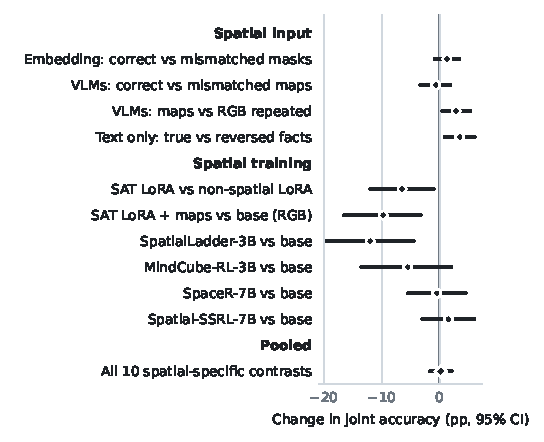
\includegraphics[width=\columnwidth]{forest_compact}
\caption{Change in EgoNormia joint accuracy (pp, 95\% CI) across spatial input and spatial training interventions, with the pooled spatial-specific effect over ten contrasts at bottom.}
\label{fig:forest}
\end{figure}

Adding the maps to the embedding (C5 vs.\ C2) raises probe accuracy by $+3.4\ [+2.2,+4.7]$ pp, so the geometry is encoded. However, while C5 improves social accuracy over C2 by $+2.6\ [+0.4,+4.9]$ pp, it does not reliably beat the mismatched-map control X1 ($+1.3\ [-0.9,+3.4]$ pp). Direct answering shows the same pattern: visual maps improve raw accuracy over RGB alone by 4 to 6 pp across the three models, but mismatched maps from unrelated videos perform equally well ($-0.7\ [-3.2,+1.8]$ pp pooled). Spatial chain-of-thought is no better than generic reasoning, and items rated as requiring high spatial understanding show no benefit ($-1.4\ [-4.6,+1.9]$ pp).

Spatial training produces an even clearer negative result. Our SAT LoRA improves held-out SAT accuracy from 78.8\% to 88.8\%, yet it falls $6.5$ pp behind the non-spatial control LoRA on EgoNormia. Published spatial models follow the same trend relative to their base checkpoints: SpatialLadder-3B changes by $-12.0\ [-19.5,-4.5]$ pp and MindCube-RL-3B by $-5.5$ pp, while SpaceR-7B ($-0.5$ pp) and Spatial-SSRL-7B ($+1.5$ pp) show little change, with larger reported spatial gains aligning with larger social losses. Combining our SAT LoRA with test-time spatial maps reduces accuracy by $9.8$ pp relative to base Qwen3-VL-8B on RGB alone, as the penalties from the adapter and the complex input simply add together without interaction.

Inspecting model predictions reveals that most differences between input conditions reflect shifts in abstention rather than social reasoning. Adding EgoNormia's own non-spatial scene description costs GPT-5.6 9 pp, entirely through extra ``None'' picks, and a mismatched description costs Qwen3-VL-32B 22 pp, whereas mismatched maps are largely ignored. When we remove ``None'' to force a substantive choice, accuracy across conditions converges (e.g., to 71.5--73.0\% for GPT-5.6), and Gemini~4's apparent gain from visual maps comes from picking ``None'' less often. Classifying wrong predictions with a GPT-5.6 judge (checked by Gemini~4) shows that only about one in 63 to 87 errors per model involves spatial geometry; roughly 60\% stem from basic perception failures and 20--31\% reflect misjudged social norms.

As supplementary context, Figure~\ref{fig:litscaling} shows the general trend across published models. We compiled these scores ourselves from public leaderboards, so the figure describes models in general rather than a finding from prior work: for the ten models reported on both the OpenCompass spatial leaderboard and the EgoNormia leaderboard, models with higher spatial scores tend to score higher on EgoNormia as well. This is what one expects when newer and larger models improve across the board, and the spatial scores closely track general ability as measured by MMMU. Capable models are good at both, but our experiments show that pushing spatial ability on its own does not make a model better at social reasoning. Our initial study remains limited by its $n{=}200$ test size, which cannot rule out effects under 3 pp, and by single-run API evaluations.

\begin{figure}[t]
\centering
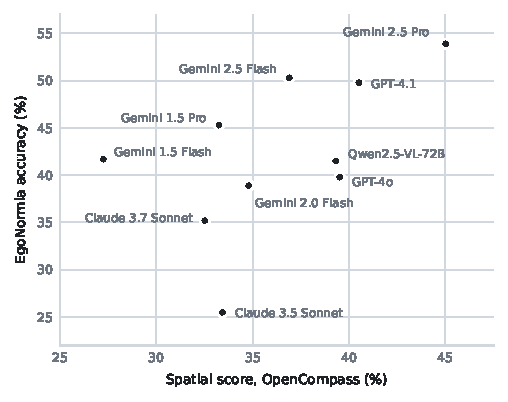
\includegraphics[width=\columnwidth]{frontier_spatial_social}
\caption{Published scores for the ten models reported in both sources: spatial score (mean of BLINK, 3DSRBench, MMSI-Bench and LEGO-Puzzles under circular evaluation; OpenCompass spatial leaderboard, 15 Aug 2025 snapshot) against EgoNormia joint accuracy (EgoNormia paper, Table~5, video models, full split).}
\label{fig:litscaling}
\end{figure}

\subsection{Updated Research Idea}
\label{sec:idea5-updated}

Our findings indicate that improving a vision-language model's spatial ability does not improve, and can even degrade, its social-norm reasoning. Because our direct evidence so far comes from a single social benchmark, a single spatial training set and a handful of models, we revise our research plan to test this null and negative transfer hypothesis across a broad grid of architectures, spatial training tasks, and social evaluations.

We will cross four factors: model scale (1B to 72B parameters), model family (Qwen-VL, InternVL, LLaVA-OneVision, and Gemma), adaptation method (LoRA, full fine-tuning, and published spatial checkpoints), and five categories of spatial training data (static SAT QA, synthetic 3D and multi-view scenes, depth and distance estimation, egocentric video spatial QA, and human pose QA). In the pose condition, we use a human-centric encoder (e.g., Meta's Sapiens2) to render keypoints and body orientations onto images while querying them in text, ensuring pose cues reach both visual and language pathways. Every spatial training run is paired with a non-spatial control matched on recipe, dataset size, and token budget so that we always measure the spatial-specific effect. A trained model enters the main analysis only if it improves on held-out spatial benchmarks (VSI-Bench, MMSI-Bench, and BLINK spatial), and we record how large that spatial gain is. We then evaluate social reasoning across EgoNormia, SIV-Bench, MuMA-ToM, MMToM-QA, EmoBench-M, and Social-IQ~2.0 under both native and forced-choice formats to eliminate abstention confounds.

Because the goal is to show that an effect is absent, a non-significant difference is not enough. Before running anything, we will fix the smallest change in social accuracy we would consider meaningful (2 pp) and choose the number of test items and seeds so that each comparison is precise enough to detect it. A spatial fine-tune then counts as showing no transfer only if the whole 90\% confidence interval of its spatial-specific effect lies within $\pm 2$ pp, which is a standard equivalence test. Across the full grid, we will also relate each run's spatial gain to its change in social accuracy while accounting for the model, data type and benchmark involved; if spatial ability drove social reasoning, runs with larger spatial gains should show larger social gains. The claim holds if no such relationship appears and the typical effect stays within the $\pm 2$ pp margin. It would be overturned by any verified spatial fine-tune whose social gain is reliably above 2 pp, replicated across seeds and at least two benchmarks, or by a clearly positive relationship between spatial gain and social change.
